\subsection{Ice temperature profile}
\chapterauthor{Kristian Sloth Lauszus and Lukas Christensen}

* Indirect: salinity, melting speed
* Drill sample
* Passive screw in the tip
	* Thermal isolated
* Measure heat conductivity of the water
	* Can be used to estimate the salinity of the water
		* Melting speed

* "back of the envelope" calculations

\begin{figure}[htb]
	\centering
	\subfloat[TODO: Caption]{
		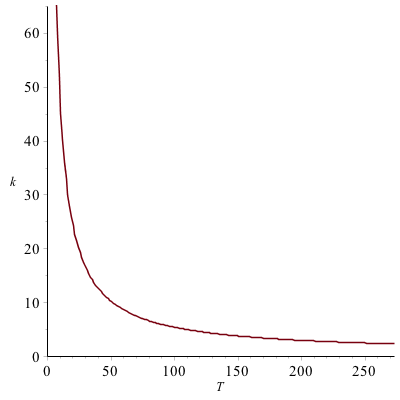
\includegraphics[width=.48\textwidth]{figures/temperature/T_vs_k.png}
	}
	\subfloat[TODO: Caption]{
		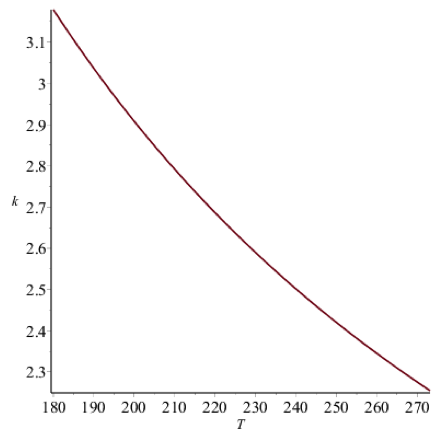
\includegraphics[width=.48\textwidth]{figures/temperature/T_vs_k_zoom.png}
	}
	\caption{TODO: Caption}
	\label{fig:T_vs_k}
\end{figure}

\begin{figure}[htb]
	\centering
	\subfloat[TODO: Caption]{
		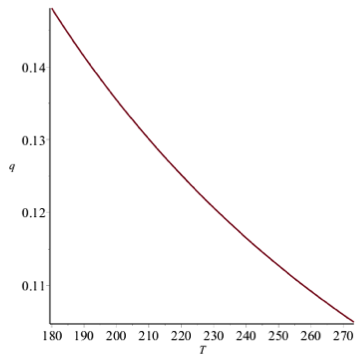
\includegraphics[width=.48\textwidth]{figures/temperature/T_vs_q.png}
	}
	\subfloat[TODO: Caption]{
		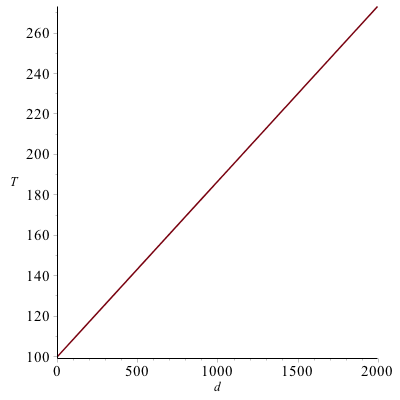
\includegraphics[width=.48\textwidth]{figures/temperature/d_vs_T.png}
	}
	\caption{TODO: Caption}
	\label{fig:T_vs_q_d_vs_T}
\end{figure}

\begin{figure}[htb]
	\centering
	\subfloat[TODO: Caption]{
		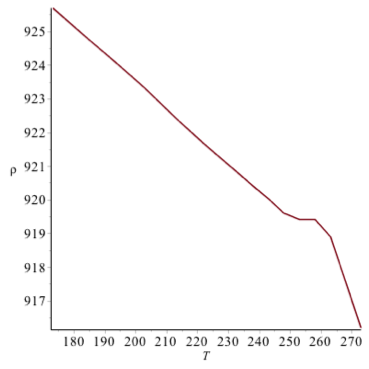
\includegraphics[width=.48\textwidth]{figures/temperature/T_vs_rho.png}
	}
	\subfloat[TODO: Caption]{
		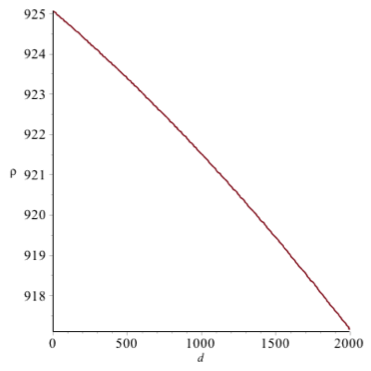
\includegraphics[width=.48\textwidth]{figures/temperature/d_vs_rho.png}
	}
	\caption{TODO: Caption}
	\label{fig:T_vs_rho_d_vs_rho}
\end{figure}

\subsubsection{Pressure Profile}

* What is the outside pressure?

\subsubsection{Simulation Results}

\subsubsection{Simulation Validation}

* Should show that the "back of the envelope" calculations are right

\begin{figure}[htb]
	\centering
	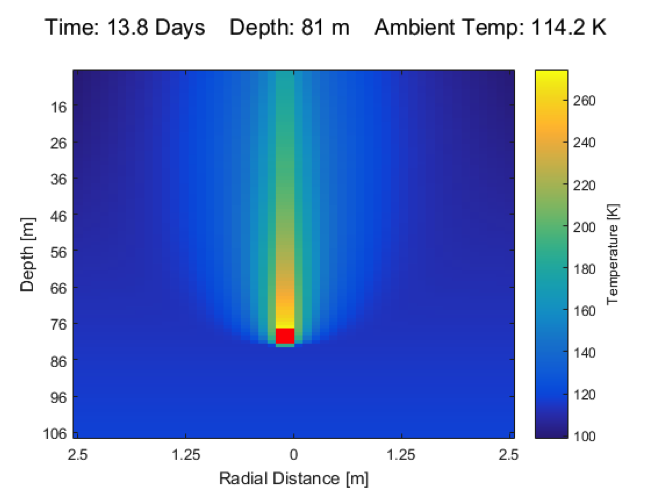
\includegraphics[width=\textwidth]{figures/temperature/temperature_simulation.png}
	\caption{TODO: Caption}
	\label{fig:temperature_simulation}
\end{figure}

\subsection{Water convection}

* Flow from tip to tail
* Passive water intake
	* Guided water intake
	* Flute shapes guides water as well
* Simulation
	* 3D model
	* CFD analysis

\begin{figure}[htb]
	\centering
	\subfloat[TODO: Caption]{
		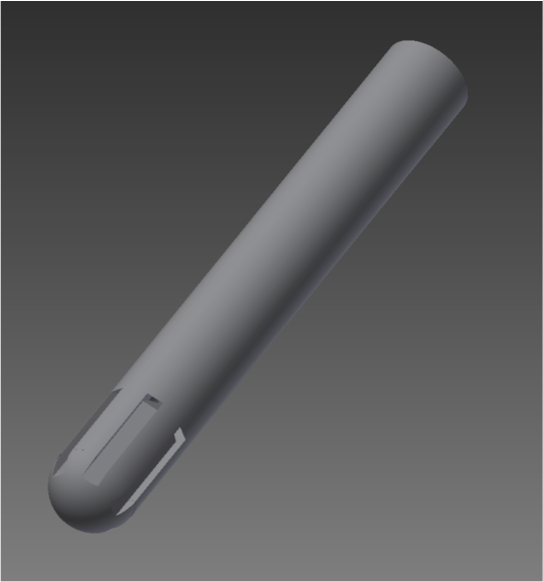
\includegraphics[width=.48\textwidth]{figures/convection/3d_model.png}
	}\\
	\subfloat[TODO: Caption]{
		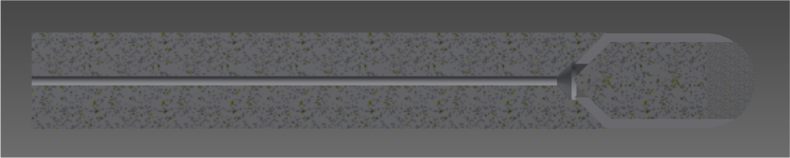
\includegraphics[width=.48\textwidth]{figures/convection/3d_model_inside.png}
	}
	\caption{TODO: Caption}
	\label{fig:3d_model}
\end{figure}

\begin{figure}[htb]
	\centering
	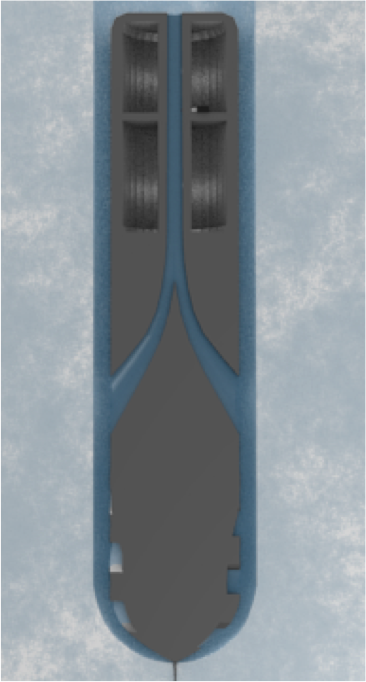
\includegraphics[width=.5\textwidth]{figures/convection/water_transportation.png}
	\caption{TODO: Caption}
	\label{fig:water_transportation}
\end{figure}

\subsubsection{CFD analysis}

* It is not enough!
	* Low Gravity!
	* 0.4 cm/s => 200 s/L
	* We will have to use a pump system

\begin{figure}[htb]
	\centering
	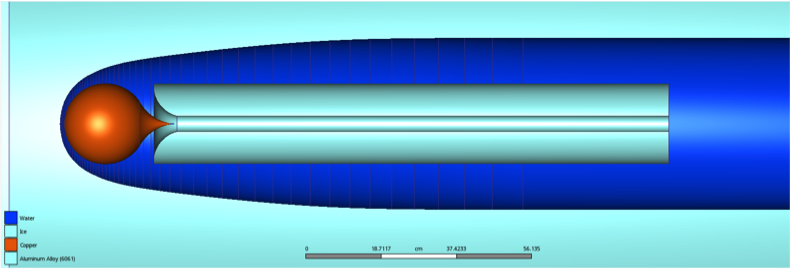
\includegraphics[width=\textwidth]{figures/convection/simplified_3d_model.png}
	\caption{TODO: Caption}
	\label{fig:simplified_3d_model}
\end{figure}

\begin{figure}[htb]
	\centering
	\subfloat[TODO: Caption]{
		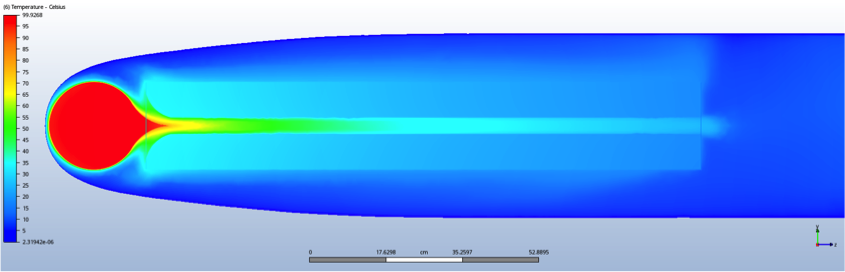
\includegraphics[width=.48\textwidth]{figures/convection/cfd_temperature.png}
	}
	\subfloat[TODO: Caption]{
		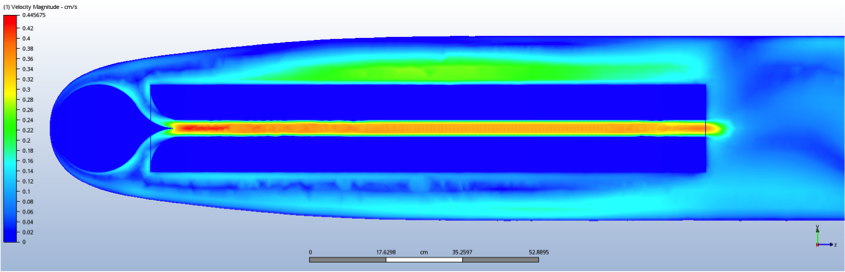
\includegraphics[width=.48\textwidth]{figures/convection/cfd_velocity.png}
	}
	\caption{TODO: Caption}
	\label{fig:cfd}
\end{figure}
